\chapter{Guiding Particle Swarms with Global Force} \label{chp:TDD}
In this chapter we want to give an introduction into the problem which we will later try to solve using reinforcement learning. Controlling large particle swarms with a global force is a challenging navigation problem. Particles can either be partially autonomous robots, which move in unison into a direction given by an external signal (e.g. a light source), or the particles can be without any autonomy where we have a global force like magnetism which controls their movement. Because particles can be seen as marbles on a surface which are controlled by tilting, the problem is often referred to as tilt problem. Depending on the task there are a number of goals which can be solved in this setting, e.g. the well-known tilt assembly problem, where the goal is to build objects using particles controlled by a global force \cite{becker2018tilt}. In this work we will focus on another problem, which finds its application in medicine and aims at navigating particles to a specific goal position inside of the human body. We will give a more detailed introduction in Section \ref{sec:TDDMotivation}. We will then continue with a theoretical point of view on the problem in Section \ref{sec:TDDPreliminaries} and present a number of existing algorithmic approaches to solve the problem in Section \ref{sec:TDDPreviousWork}. We will finally present previous work on solving the problem with reinforcement learning in Section \ref{sec:TDDRL}. 

\section{Motivation} \label{sec:TDDMotivation}
The treatment of medical problems often requires the use of some sort of medication. These medications are given as oral ingestion or intravascular  injection and then are further distributed throughout the body via blood circulation. Most if not all of these treatments can produce some potentially serious unwanted side-effects. Especially when treating serious medical problems like internal bleedings, localized infections, tumors or cancer (see Figure \ref{fig:brain_tumor}), a large portion of the medication does not reach its target destination and the possible worst-case side-effects can be as serious as the original medical problem. The idea of \textit{targeted drug delivery}, aims at concentrating some given medicine in a certain part of the body to reduce unwanted side-effects and at the same time increase the efficacy.

\begin{figure}[ht]
    
    \begin{center}
        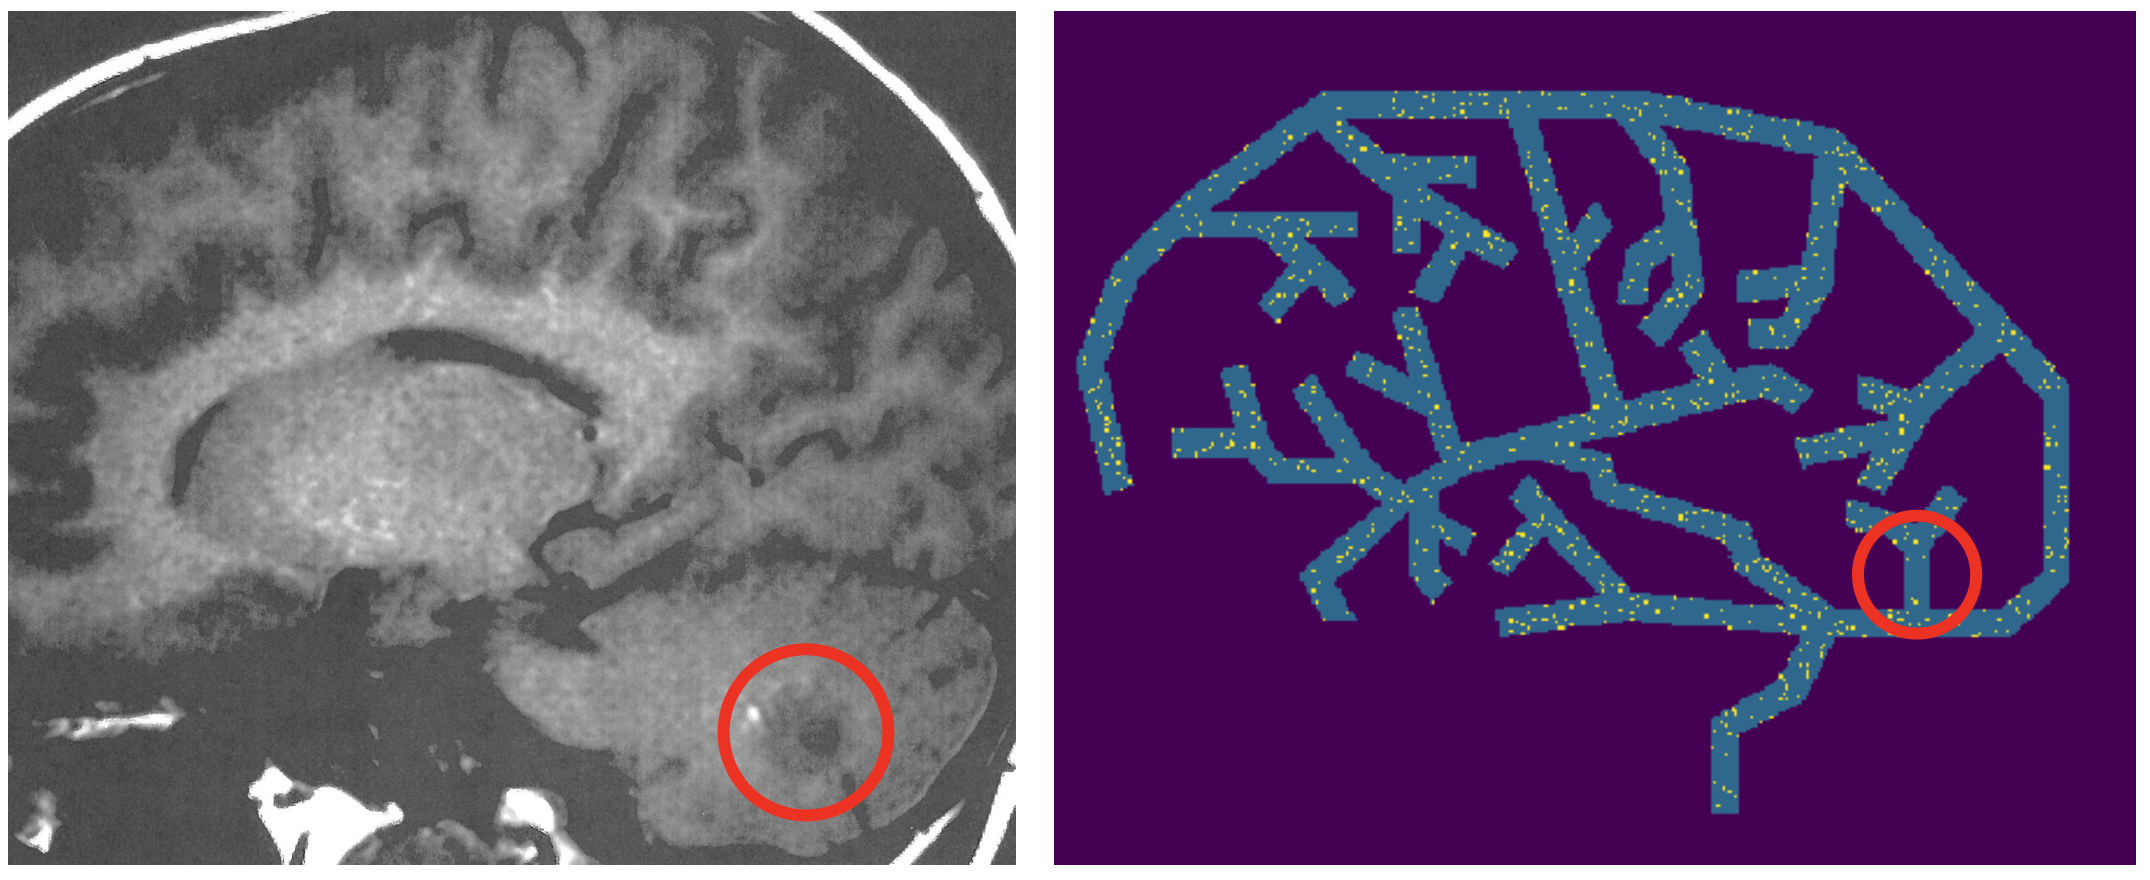
\includegraphics[clip, width=0.7\columnwidth]{figures/drugdelivery/brains.png}
    \end{center}
    
    %\vspace*{-6pt}
    \caption[Targeted Drug Delivery Example]{Targeted drug delivery for tumor treatment (from \cite{becker2020}). An MRI image on the right shows a tumor (marked by the red circle) and an abstracted version (left) shows particles containing some sort of medicine (yellow dots) which should be delivered to the target region.}
    \label{fig:brain_tumor}
    %\vspace*{-12pt}
\end{figure}

Over the years many approaches have been developed to perform targeted drug delivery. In recent work, the idea of using magnetic nanoparticles has been explored and proven to be promising, since they combine high drug loading with great targeting abilities \cite{vangijzegem2019magnetic, albinali2019perspective}. The particles are controlled by an external uniform magnetic force and guided towards a target location. The magnetic fields can be generated by using modified coils in an \textit{Magnetic Resonance Imaging} (MRI) scanner \cite{mathieu2007magnetic, mellal2015magnetic}. Real-time MRI scanning also allows particle localization and feedback control to some extend \cite{pouponneau2009magnetic}. At their target location, the particles are activated to release their payload by an external or internal stimulus such as temperature or pH.

Guiding particles by a uniform (\textit{global}) force requires solving a complex distributed navigation problem. The nanoparticles will be distributed randomly in a complex maze-like environment given by the vascular system of blood vessels. Guiding all particles regardless of their initial position to a single destination will be complicated due to many particles colliding at some point with obstacles. However the underlying algorithmic problem does not need to include the goal position as moving a single particle to a goal position is easy. We therefore can reduce the problem to finding a gathering sequence, which concentrates all particles in a single point. We can then move all particles together to the goal position. 

This problem has been studied in the past in terms of bringing two particles to the same location called \textit{symmetric rendezvous search} \cite{anderson2001two,alpern2006theory}. The strategies were originally designed for agents with were able to make onboard computations, but are still applicable to particles since some cases proposed symmetric moving protocols where each agent executes the same movement (except when being blocked by an obstacle). By successively applying a strategy which merges two particles, all particles can be gathered and brought to the goal position together. 

In this chapter we want to focus on recent work by Becker et al. \cite{becker2020}. They proved that the underlying problem of finding an optimal gathering sequence is NP-hard and also present some novel approximation algorithms which greatly improve previous worst case guarantees. They also propose to use reinforcement learning to solve the problem and show, that the results are better than the results of their approximation algorithms for a set of test instances.

\section{Preliminaries} \label{sec:TDDPreliminaries}
Using particles with individual capabilities (e.g. microrobots) is difficult since the tiny volume of these robots makes it nearly impossible to store enough energy to navigate in presence of flowing blood. The particles we are dealing with therefore have no computational power, memory or any other autonomy. Instead our particles are just some kind of substrate (e.g. iron-oxide) injected into the blood vessels and solely controlled by a uniform global force which affects all particles equally. In our model we will work with a two-dimensional abstraction of the environment and the particles: The blood-vessels will be modeled by a planar two-dimensional integer workspace $P$ which consists of orthogonal cells (\textit{pixels}) and can therefore be seen as \textit{polyomino}. All pixels not belonging to the polyomino are blocked and cannot be entered by particles. The distance $dist(p, q)$ between two pixels $p$ and $q$ is given by the shortest path on the integer grid between $p$ and $q$ that stays within $P$. The diameter $D$ of the polyomino is then given by the maximum distance between any two of its pixels. 

At the beginning, each pixel of $P$ may contain one (or more) particles which we will call the \textit{configuration} of $P$, with the set of all possible configurations $\mathcal{P}$. Since we are dealing with edge-to-edge connected cells, four basic moves are possible to move each particle by one cell in one of the directions "Up" (\textit{u}), "Down" (\textit{d}), "Left" (\textit{l}) or "Right" (\textit{r}). If the particle cannot move to the next cell because it is blocked, it simply remains in its current cell. Since the size of the particles is insignificant compared to the size of the cells, if two particles $a$ and $b$ enter the same cell $p$, they will merge into a single particle. This can happen when $a$ enters $p$, while $b$ remains in $p$ due to being blocked. Merged particles will never be separated again and move in unison for subsequent moves.

We call a series of commands a \textit{motion plan} $C = \langle c_1, c_2, c_3, \dots \rangle$ where each command $c_i \in \{u, d, l, r\}$. We further call a command sequence \textit{gathering} if it merges all particles of a given configuration $A \in \mathcal{P}$ into a single pixel, such that $|A'| = 1$.


\section{Algorithmic Approaches} \label{sec:TDDPreviousWork}
In this Section we want to present a number of algorithmic approaches to solve targeted drug delivery. To keep things short, we will focus on recent algorithms which provide a reasonably good performance bound and have proven to perform at least as good as previous approaches. All algorithmic approaches use a gathering strategy, which first concentrates all particles into a single cell. The particles are then guided to the target area on a shortest path.

\subsection{Static Shortest Path}
In 2016 Mahadev et al. developed a simple greedy algorithm which is able to collect all $m$ particles with a command sequence of length $\mathcal{O}(m \cdot n^3)$, where $n$ is the polyomino's height times its width \cite{mahadev2016collecting}. The algorithm was later named \textit{Static Shortest Path} (SSP) in a paper by Becker et al. \cite{becker2020}. 

\begin{algorithm}[ht]
    \KwData{Configuration $A$, Bounded polyomino $P$}

    \While{$|A| > 1$}{
        Select two particles $a$ and $b$ from $A$. \;
        \texttt{StaticShortestPath}($a$, $b$)
    }

    \SetKwProg{Merge}{procedure}{:}{}
    \Merge{\texttt{StaticShortestPath} ($a$ : Particle, $b$: Particle)}{
        \While{$dist(a, b) \neq 0$} {
        Compute $C \in \{u, d, l, r\}^N$ as the shortest control sequence to move $a$ onto $pos(b)$. \;
        Execute $C$.
        }
    }
    
    \caption[Static Shortest Path Algorithm]{The static shortest path algorithm modified to merge an arbitrary number of particles.} \label{alg:SSP}
\end{algorithm}

The algorithm works by iteratively merging two particles until all particles are merged into a single one. We included a sketch in Algorithm \ref{alg:SSP}. We can see, that the algorithm uses the procedure \texttt{StaticShortestPath}, which subsequently moves a particle $a$ to the position of another particle $b$ until they are merged. Mahadev et al. showed, that when moving $a$ to the position ob $b$, the distance between the particles $a$ and $b$ only decreases if $b$ had a collision. Since the polyomino is bounded and $a$ and $b$ always move into the same direction, $b$ must have a collision after $\mathcal{O}(n)$ collision free iterations. Therefore $\mathcal{O}(n^2)$ commands are needed to reduce the distance by at least one, resulting in $\mathcal{O}(n^3)$ commands in total to merge two particles. The choice of particles that are merged in the next step can be random, but it has been shown, that choosing the pair with the maximal distance converges faster on average.

\subsection{Dynamic Shortest Path}
In 2020, Becker et al. presented a number of improved algorithms which provide stronger performance bounds \cite{becker2020}. For the special case of hole-free polyominos, they developed the \textit{Dynamic Shortest Path} (DSP) algorithm which is able to compute a gathering sequence of $\mathcal{O}(D)$ with $D$ being the diameter of the polyomino. For non-simple polyominos, DSP still always merges two particles, but may need $\mathcal{O}(nD)$ steps, where $n$ is the number of pixels in the polyomino. 

\begin{figure}[ht]
    
    \begin{center}
        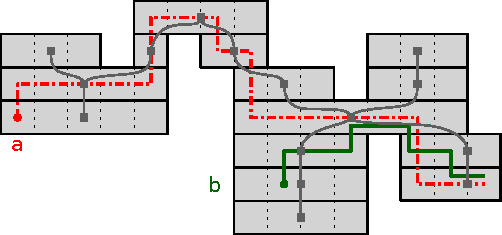
\includegraphics[clip, width=0.6\columnwidth]{figures/drugdelivery/Gathering_Simple_b.pdf}
    \end{center}
    
    %\vspace*{-6pt}
    \caption[DSP and the Edge Contact Graph]{A simple polyomino $P$ and its edge-contact graph $\mathcal{C}(R)$. The particle $a$ (red) is moved towards particle $b$ (green) on a shortest path with respect to $\mathcal{C}(R)$. (from \cite{becker2020}, edited)}
    \label{fig:edge_contact_graph}
    %\vspace*{-12pt}
\end{figure}


\begin{algorithm}[ht]
    \KwData{Configuration $A$, Bounded polyomino $P$}

    \While{$|A| > 1$}{
        Select two particles $a$ and $b$ from $A$. \;
        \texttt{DynamicShortestPath}($a$, $b$)
    }

    \SetKwProg{Merge}{procedure}{:}{}
    \Merge{\texttt{DynamicShortestPath} ($a$ : Particle, $b$: Particle)}{
        \While{$R^a_t \neq R^b_t$} {
            Compute a shortest path $S_t$ from $R^a_t$ to $R^b_t$ in $\mathcal{C}(R)$ \;
            Move $a$ to $S_t(1)$ via a shortest path in $P$. \;
            Update $R^a_t$ and $R^b_t$
        }

        Compute a shortest path $C$ from $a$ to $b$. \;
        Merge $a$ and $b$ by executing $C$.
    }
    
    \caption[Dynamic Shortest Path Algorithm]{The dynamic shortest path algorithm modified to merge an arbitrary number of particles.}\label{alg:DSP}
\end{algorithm}

The DSP algorithm starts by decomposing $P$ with horizontal lines through pixel edges which results in a set of rectangles $R$. The edge-contact graph $\mathcal{C}(R)$ is then constructed by creating a vertex for each rectangle and connecting two vertices if their respective rectangles share an edge. For a simple (hole-free) polyomino the edge-contact graph is a tree. Two particles are then merged by using an improved shortest path strategy. For two particles $a$ and $b$, let $R^a_t$ and $R^b_t$ be the rectangles of $P$ containing the two particles in step $t$. Let $S_t$ be a shortest path from $R^a_t$ to $R^b_t$ and let $S_t(1)$ be the successor of $R^a_t$ on $S_t$ if it exists ($R^a_t \neq R^b_t$). The particles are then merged, by subsequently moving $a$ on a shortest path from $R^a_T$ to $S_t(1)$ and then recalculating $S_t$ (therefore the name \textit{dynamic} shortest path). If there is no $S_t(1)$ the particles are merged, by moving $a$ towards $b$ by a shortest (horizontal) path, merging both particles within $R^a_t$. The whole process can be found in Algorithm \ref{alg:DSP} and an example showing the edge-contact graph and the process of merging two particles is shown in Figure \ref{fig:edge_contact_graph}.


\subsection{Move to Extremum}
The strategy \textit{Move to Extremum} (MTE) was also developed by Becker et al. \cite{becker2020} and provides a strategy which - independent of the shape of the polyomino - provides a gathering sequence of length at most $\mathcal{O}(D^2)$ for two particles. The idea of MTE is to iteratively move an extreme particle (e.g. the top-rightmost) to an opposite extremum (e.g. bottom-leftmost) along a shortest path. Similar to the shortest path approach in SSP, the distance then decreases with every iteration. 

Let $q$ be the top-rightmost pixel of $P$. To merge two particles, we select the bottom-leftmost particle $a$ and compute a sequence of moves, which moves $a$ to $q$ on a shortest path. We repeat this procedure of selecting the bottom-leftmost particle and moving it to $q$ until the particles have been merged. In each iteration, the sum of distances $\Delta$ of the two particles to $q$ decreases. This happens only if the other particle $b$ has a collision. Similarly to SSP, in every iteration the particle $b$ must have at least one collision (otherwise $q$ could not be the top-rightmost pixel or $a$ not the bottom-leftmost particle), so the sum decreases at least by 1 every $D$ steps. Since in some polyominos (e.g. a square), the number of pixels $n$ is in $\Omega (D^2)$, we can argue, that the MTE produces sequences which are significantly shorter than $\mathcal{O}(n^3)$ from SSP.

\begin{algorithm}[ht]
    \KwData{Configuration $A$, Bounded polyomino $P$}
    
    Determine which of the four corner types occurs at most $k/4$ times. \;
    Apply a sequence of commands to merge all particles into at most $k/4$ groups.

    \While{$|A| > 1$}{
        Calculate the sum of distances for all particles $d_t$ for each extremum. \;
        For each command calculate the change in the sum of distances $\Delta d_t^{c_i}$ that command would produce. \;
        Select the command $j$ which decreases the sum the most. \;
        \eIf{$\Delta d_t^{c_j} < 0$}{
            Execute $j$
        }{
            Select two particles $a$ and $b$ from $A$. \;
            \texttt{MoveToExtremum}($a$, $b$)
        }
    }

    \SetKwProg{Merge}{procedure}{:}{}
    \Merge{\texttt{MoveToExtremum} ($a$ : Particle, $b$: Particle)}{
        Select an extremum $q$ which minimizes the sum to $a$ and $b$. \;
        \While{$dist(a, b) \neq 0$} {
            Select the particle which is further away from $q$. \;
            Move that particle to $q$ on a shortest path. \;
        }

    }
    
    \caption[The Min Sum To Extremum algorithm]{The min sum to extremum algorithm to gather all particles. MTE is used as a subroutine and particles are merged into $k/4$ groups in convex corners at the beginning to reduce their total number.}\label{alg:MSTE}
\end{algorithm}

If we look at a swarm of particles, we can have at most $n$ individual particles in any configuration of a polyomino $P$, which would result in a total of $\mathcal{O}(nD^2)$ commands for a gathering sequence using MTE. Luckily, it is possible to further reduce the total number of particles by first moving them into convex corners. For every polyomino with $k$ convex corners, a diameter $D$ and a configuration $A \in \mathcal{P}$, this can be done with a command sequence of length $2D$. The resulting configuration $A' \in \mathcal{P}$ will have at most $k/4$ particles. This works by first selecting the type of convex corner from all convex corners (northwest (NW), northeast (NE), southwest (SW) and southeast (SE)) which occurs at most $k/4$ times. It is guaranteed by the pigeon hole principle that such a convex corner type must exist. Let us assume the NE corner is the type selected. After applying a sequence of $\langle r, u \rangle^D$ every particle lies in a NE corner. Therefore the total gathering sequence of MTE has a length of $\mathcal{O}(kD^2)$. 

In their paper, Becker et al. also propose a variant of MTE called \textit{Min Sum To Extremum} (MSTE) which generalizes the idea of MTE for a swarm of particles. Initially, MTE selects an extremum which has the smallest sum of distances to all particles. It then tries to find a command which reduces this sum the most. If it is unable to find such a command, it continues by merging two particles using regular MTE. We provide pseudocode for MSTE which also includes MTE as a subroutine in Algorithm \ref{alg:MSTE}. The particles are gathered into $k/4$ groups at the beginning.

\section{The Reinforcement Learning Approach} \label{sec:TDDRL}
In 2019 Li Huang showed that is is possible to solve the targeted drug delivery problem with reinforcement learning \cite{huang2019}. His approach was later tested against the algorithmic approaches and proved to significantly outperform both MTE and MSTE on individual instances \cite{becker2020}. In this section, we want to give an overview over how the agents for targeted drug delivery can be trained. The methods and terminology which are used for this approach will be explained in detail in Chapter \ref{chp: RLOverview}.

\begin{figure}[ht]
    
    \begin{center}
        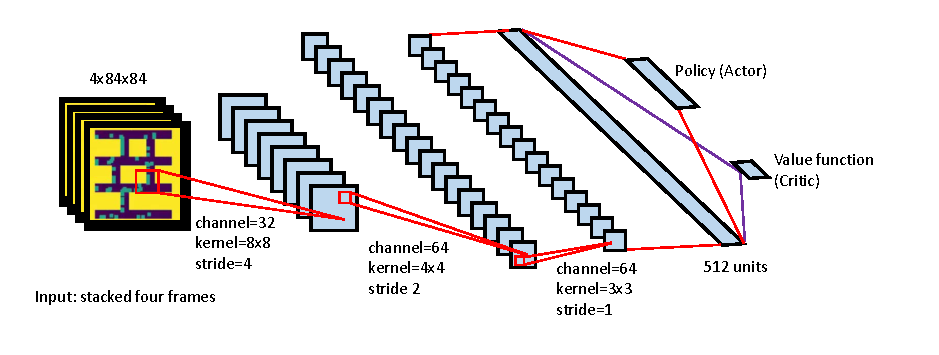
\includegraphics[clip, width=0.95\columnwidth]{figures/drugdelivery/Network_Architecture.pdf}
    \end{center}
    
    %\vspace*{-6pt}
    \caption[Network Architecture for the RL Approach]{The network architecture for the reinforcement learning approach (from \cite{huang2019}).}
    \label{fig:huang_network_architecture}
    %\vspace*{-12pt}
\end{figure}

\paragraph{The Particle Maze Environment.}
For reinforcement learning every problem has to be modeled as an environment where the agent can take actions and from where it receives observations and reward in return. For the problem of gathering particles at a goal location, the environment represents a single instance of the targeted drug delivery problem (a single polyomino) with a single target position. Particles are randomly spawned in empty cells of the polyomino at the beginning of an episode and the episode ends if all particles reach the goal position or after a certain time limit. Observations are generated as a visual representation of the environment as a grayscale image. The image includes the shape of the polyomino and the position of each particle. The observation will the be further preprocessed by downscaling the image to $84 \times 84$ pixels. Additionally the network receives a stack of the last four frames to add information about past particle positions. Images are also normalized by their variance and zero centered with precomputed values from a random agent playing 10000 steps.

For reinforcement learning, the reward signal is a crucial component. Even a simple problem might become very hard to learn for an agent if the reward signal does not provide enough information about the goal or if it is somehow inconsistent or extremely sparse. Huang et al. generated reward based on a set of predefined goals. There are two main categories for these goals: The maximum distance of any particle to the goal position and the average distance of all particles to the goal position. In each category, the agent receives rewards based on reaching certain milestones - e.g. if the particle with the largest distance to the goal is less than 50 cells away from the goal position, the agent is granted a reward of $+2$. Rewards may increase for higher goal tiers and are only granted a single time for each episode. If the agent is able to bring all particles to the goal position it receives a large final reward of $+100$. The goals that were used during the experiments were sparse and limited to only 4-8 distinct rewards in each category. Rewards are also not normalized.

\begin{table} [ht]
    \begin{center}
        \begin{tabular}{|p{6.5cm}|c|}
            \hline
            Hyperparameter & Default Value \\
            \hline
            Extrinsic Reward Clipping & False \\
            Extrinsic Reward Normalization & False \\
            Intrinsic Reward Clipping & False \\
            Intrinsic Reward Normalization & True \\
            Steps Per Episode & 2048 \\
            Total Steps & 2e8 \\
            Number of Minibatches & 16 \\
            Number of optimization epochs & 4 \\
            Extrinsic Reward Coefficient & 1.0 \\
            Intrinsic Reward Coefficient & 0.5 \\
            Number of Environments & 128 \\
            Learning Rate & 0.0001 \\
            Entropy Coefficient & 0.001 \\
            \hline
        \end{tabular}
    \end{center}
    \caption[RL Approach Default Parameters]{Default parameters for PPO with RND curiosity rewards as used in the reinforcement learning approach on the targeted drug delivery problem by Huang and Becker et al. \cite{huang2019}.} \label{tab:RLDefaults}
\end{table}

\paragraph{The Targeted Drug Delivery Agent}
The agent for the targeted drug delivery problem is inspired by the agent used for the large scale study on curiosity learning by Burda et al. in 2018 \cite{burda2018large}. Since the targeted drug delivery problem requires careful exploration of the environment, the agent heavily profits from the addition of a curiosity reward. For reward generation the original methods from \cite{burda2018large} were used, as well as the random network distillation method (see Section \ref{ssec:Curiosity}). RND showed superior performance in all experiments which were done with both rewards. 

The agent itself is build with an actor-critic architecture and trained using the PPO algorithm (see Section \ref{ssec:PPO}). The neural network uses convolutional layers to process the image information (see Section \ref{ssec:CNNs}) and follows the frequently used natural CNN design. The architecture can be found in Figure \ref{fig:huang_network_architecture} and consists out of three convolutional layers with 32 ($8\times 8, s=4$), 64 ($4\times 4, s=2$) and 64 ($2\times 2, s=1$) filters which are then connected to a single fully connected layer with 512 neurons. The original four commands used to move the particles are extended by another four additional commands. Rather than just using "North" (up), "South" (Down), "West" (Right) and "East" (Left), the agent also is allowed to also use "Northwest", "Northeast", "Southwest" and "Southeast" as movement commands. Additional training parameters for PPO and curiosity can be found in Table \ref{tab:RLDefaults}.

The reinforcement learning approach proved to have exceptionally good performance on single (small) instances, but is costly due to the long training process. Huang et al. showed, that PPO was not able to successfully solve instances by using the extrinsic reward signal only. Even after extremely long training sessions with over 3 billion timesteps, PPO was not able to solve a single instance. The addition of the intrinsic curiosity reward solved this problem, by dramatically decreasing training time and leading to positive results even for larger and more complex instances.
